\documentclass[11pt,a4paper]{article}
\usepackage[utf8]{inputenc}
\usepackage[margin=0.8in]{geometry}
\setlength{\headheight}{14pt}
\usepackage{graphicx}
\usepackage{amsmath,amssymb}
\usepackage{booktabs}
\usepackage{longtable}
\usepackage{array}
\usepackage{hyperref}
\usepackage{float}
\usepackage{caption}
\usepackage{subcaption}
\usepackage{fancyhdr}
\usepackage{titlesec}
\usepackage{xcolor}

% Custom Colors matching previous reports
\definecolor{primary}{RGB}{0, 51, 102}
\definecolor{secondary}{RGB}{70, 130, 180}

\hypersetup{
    colorlinks=true,
    linkcolor=primary,
    citecolor=primary,
    urlcolor=secondary
}

% Header and Footer setup
\pagestyle{fancy}
\fancyhf{}
\rhead{\textcolor{primary}{\textbf{EDC Laboratory --- Experiment 4}}}
\lhead{\textcolor{primary}{\textbf{EE25BTECH11056 \& EE25BTECH11049}}}
\rfoot{Page \thepage}

\titleformat{\section}{\large\bfseries\color{primary}}{\thesection.}{0.5em}{}
\titleformat{\subsection}{\normalfont\bfseries\color{secondary}}{\thesubsection}{0.5em}{}
\titleformat{\subsubsection}{\normalfont\bfseries}{\thesubsubsection}{0.5em}{}

\begin{document}

% Title Page / Header Block
\begin{center}
    {\LARGE \textbf{\color{primary} DEPARTMENT OF ELECTRICAL ENGINEERING}}\\[0.2cm]
    {\large \textbf{Electronic Devices \& Circuits Laboratory (EDC LAB)}}\\[0.4cm]
    \rule{\linewidth}{1pt}\\[0.3cm]
    {\Large \textbf{EXPERIMENT 4: NMOS Common-Source Amplifier with Resistive Load: DC Transfer Characteristic and Small-Signal Gain}}\\[0.3cm]
    \rule{\linewidth}{1pt}\\[0.4cm]
    
    \begin{tabular}{ll}
        \textbf{Prepared By:} & \textbf{Suraj.N (EE25BTECH11056)} \\
                              & \textbf{Sai Krishna Bakki (EE25BTECH11049)} \\
        \textbf{Course:}      & Electronic Devices \& Circuits Lab \\
        \textbf{Date:}        & \today
    \end{tabular}
\end{center}

\vspace{0.3cm}

\section{Aim and Objectives}
\begin{enumerate}
    \item To construct an N-channel enhancement MOSFET (2N7002 / 2N7000) Common-Source (CS) amplifier with a resistive drain load ($R_D$).
    \item To measure, record, and plot its full \textbf{DC Transfer Characteristic} ($V_{\text{OUT}}$ vs $V_{\text{IN}}$) by sweeping $V_{\text{IN}}$ from $0\text{ V}$ to $2.4\text{ V}$ under a supply voltage $V_{DD} = 10\text{ V}$, identifying the cutoff, saturation (amplification), and triode regions.
    \item To extract the small-signal voltage gain $A_v(V_{\text{IN}})$ as a function of the DC bias point using two independent methods:
    \begin{itemize}
        \item \textbf{Method 1 (Numerical Slope):} Differentiating the measured DC transfer curve:
        \begin{equation*}
            A_v(V_{\text{IN}}) = \frac{dV_{\text{OUT}}}{dV_{\text{IN}}}
        \end{equation*}
        \item \textbf{Method 2 (Direct AC Measurement):} Superposing a sinusoidal test tone ($v_{\text{in}} = 10\text{ mV}$ amplitude, $f = 1\text{ kHz}$) through a $C = 0.1\ \mu\text{F}$ coupling capacitor, sweeping the DC bias offset via a $1\text{ M}\Omega$ isolation resistor from $0\text{ V}$ to $1.8\text{ V}$, and measuring the AC output response ($V_{\text{OUT(RMS)}}$).
    \end{itemize}
    \item To evaluate the correlation between large-signal slope and small-signal gain, and to thoroughly analyze the underlying semiconductor physics across the operating regions.
\end{enumerate}

\section{Apparatus and Software Tools Required}
\begin{table}[H]
\centering
\caption{Equipment, Components, and Simulation Tools Used}
\begin{tabular}{cp{4.5cm}p{6.8cm}c}
\toprule
\textbf{S.No.} & \textbf{Component / Equipment} & \textbf{Specification / Value} & \textbf{Quantity} \\
\midrule
1 & N-Channel MOSFET & 2N7002 / 2N7000 & 1 \\
2 & Drain Load Resistor ($R_D$) & $10\text{ k}\Omega$ (Part A) / $300\text{ k}\Omega$ (Part B) & 1 each \\
3 & DC Bias Isolation Resistor & $1\text{ M}\Omega$ (Part B) & 1 \\
4 & AC Coupling Capacitor & $0.1\ \mu\text{F}$ ceramic/film & 1 \\
5 & Regulated Dual DC Power Supply & $0\text{--}30\text{ V}$ (for $V_{DD} = 10\text{ V}$ and variable DC bias) & 1 \\
6 & Function / Signal Generator & Sine Wave, $10\text{ mV}$ peak ($20\text{ mV}_{\text{pp}}$), $1\text{ kHz}$ & 1 \\
7 & Digital Oscilloscope / DMM & AC RMS \& peak-to-peak voltage measurement & 1 \\
8 & Simulation Software & LTspice XVII & -- \\
\bottomrule
\end{tabular}
\end{table}

\section{Overall Theoretical Framework}
In a Common-Source (CS) NMOS amplifier with a resistive drain load $R_D$, the input voltage $V_{\text{IN}}$ is applied between the gate and source terminals ($V_{GS} = V_{\text{IN}}$), while the output voltage $V_{\text{OUT}}$ is taken at the drain node ($V_{DS} = V_{\text{OUT}} = V_{DD} - I_D R_D$).

Depending on the magnitude of $V_{\text{IN}}$ relative to the device threshold voltage ($V_T$) and the drain voltage $V_{\text{OUT}}$, the transistor traverses three distinct operational regions:
\begin{enumerate}
    \item \textbf{Cut-off Region ($V_{\text{IN}} < V_T$):}
    \begin{equation}
        I_D = 0 \implies V_{\text{OUT}} = V_{DD} - 0 \cdot R_D = V_{DD}
    \end{equation}
    The output remains pinned at the positive rail ($V_{DD} = 10\text{ V}$). The incremental transconductance is zero ($g_m = 0$), yielding zero small-signal gain:
    \begin{equation}
        A_v = \frac{dV_{\text{OUT}}}{dV_{\text{IN}}} = 0
    \end{equation}

    \item \textbf{Saturation Region ($V_{\text{IN}} \ge V_T$ and $V_{\text{OUT}} \ge V_{\text{IN}} - V_T$):}
    The inversion channel pinches off before reaching the drain terminal. The drain current obeys the classic square-law relation:
    \begin{equation}
        I_D = \frac{1}{2} k_n (V_{\text{IN}} - V_T)^2 (1 + \lambda V_{\text{OUT}}) \approx \frac{1}{2} k_n (V_{\text{IN}} - V_T)^2
    \end{equation}
    The corresponding DC output voltage drops quadratically as $V_{\text{IN}}$ increases:
    \begin{equation}
        V_{\text{OUT}} = V_{DD} - \frac{1}{2} k_n R_D (V_{\text{IN}} - V_T)^2
    \end{equation}
    The voltage gain is given by the derivative:
    \begin{equation}
        A_v = \frac{dV_{\text{OUT}}}{dV_{\text{IN}}} = - k_n R_D (V_{\text{IN}} - V_T) = - g_m R_D
    \end{equation}
    Because $g_m = k_n (V_{\text{IN}} - V_T) = \sqrt{2 k_n I_D}$ increases linearly with gate overdrive voltage $(V_{\text{IN}} - V_T)$, the magnitude of the small-signal gain $|A_v|$ rises steeply as $V_{\text{IN}}$ increases, reaching its maximum right at the boundary between saturation and triode.

    \item \textbf{Triode (Linear / Ohmic) Region ($V_{\text{IN}} \ge V_T$ and $V_{\text{OUT}} < V_{\text{IN}} - V_T$):}
    When $I_D R_D$ becomes sufficiently large, $V_{\text{OUT}}$ drops below the pinch-off threshold ($V_{DS} < V_{GS} - V_T$). The inversion channel extends continuously from source to drain, and the current is governed by:
    \begin{equation}
        I_D = k_n \left[ (V_{\text{IN}} - V_T) V_{\text{OUT}} - \frac{1}{2} V_{\text{OUT}}^2 \right]
    \end{equation}
    As $V_{\text{IN}}$ is swept further, the transistor acts as an increasingly low on-resistance channel ($r_{ds,\text{on}} \approx \frac{1}{k_n(V_{\text{IN}} - V_T)}$). $V_{\text{OUT}}$ collapses towards $0\text{ V}$, flattening the transfer curve and causing the gain $A_v = \frac{dV_{\text{OUT}}}{dV_{\text{IN}}} \to 0$.
\end{enumerate}

\clearpage

% =========================================================================
% PART A
% =========================================================================
\section{Part A: DC Transfer Characteristic (VOUT vs VIN)}

\subsection{Circuit Description and LTspice Simulation}
In Part A, the NMOS gate is driven directly by a variable DC voltage source ($V_{\text{IN}}$), swept from $0\text{ V}$ to $2.4\text{ V}$. The drain is tied to $V_{DD} = 10\text{ V}$ through a load resistor $R_1 = 10\text{ k}\Omega$, and the source is grounded. Figure~\ref{fig:part_a_schematic} displays the LTspice schematic, and Figure~\ref{fig:part_a_sim} shows the simulated DC transfer characteristic ($V(n001)$ vs $V_{\text{IN}}$).

\begin{figure}[H]
    \centering
    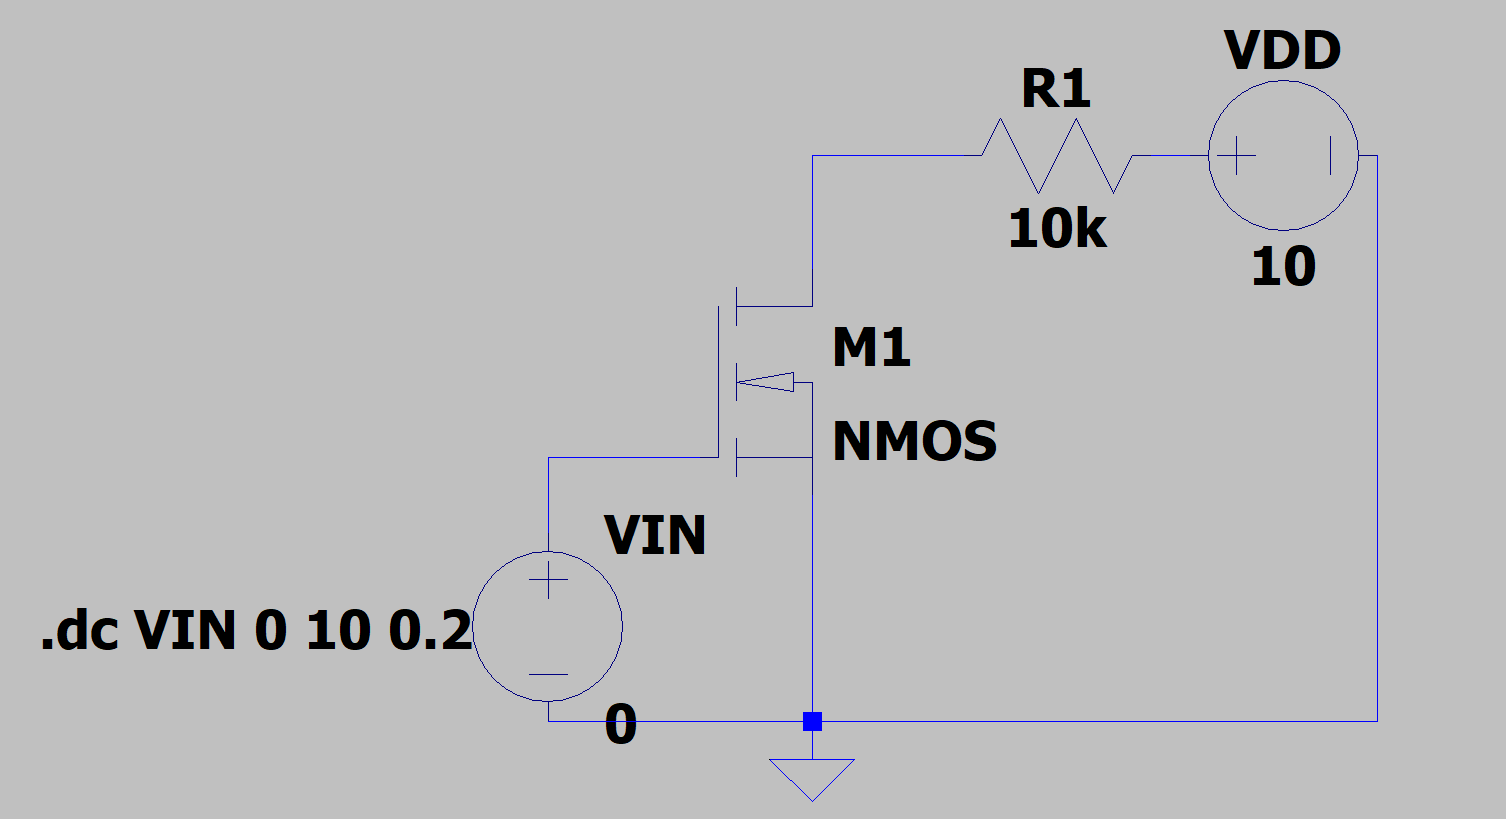
\includegraphics[width=0.55\textwidth]{../Schematic_a.png}
    \caption{Part A: Circuit Schematic of NMOS CS Amplifier with $R_D = 10\text{ k}\Omega$ and $V_{DD} = 10\text{ V}$.}
    \label{fig:part_a_schematic}
\end{figure}

\begin{figure}[H]
    \centering
    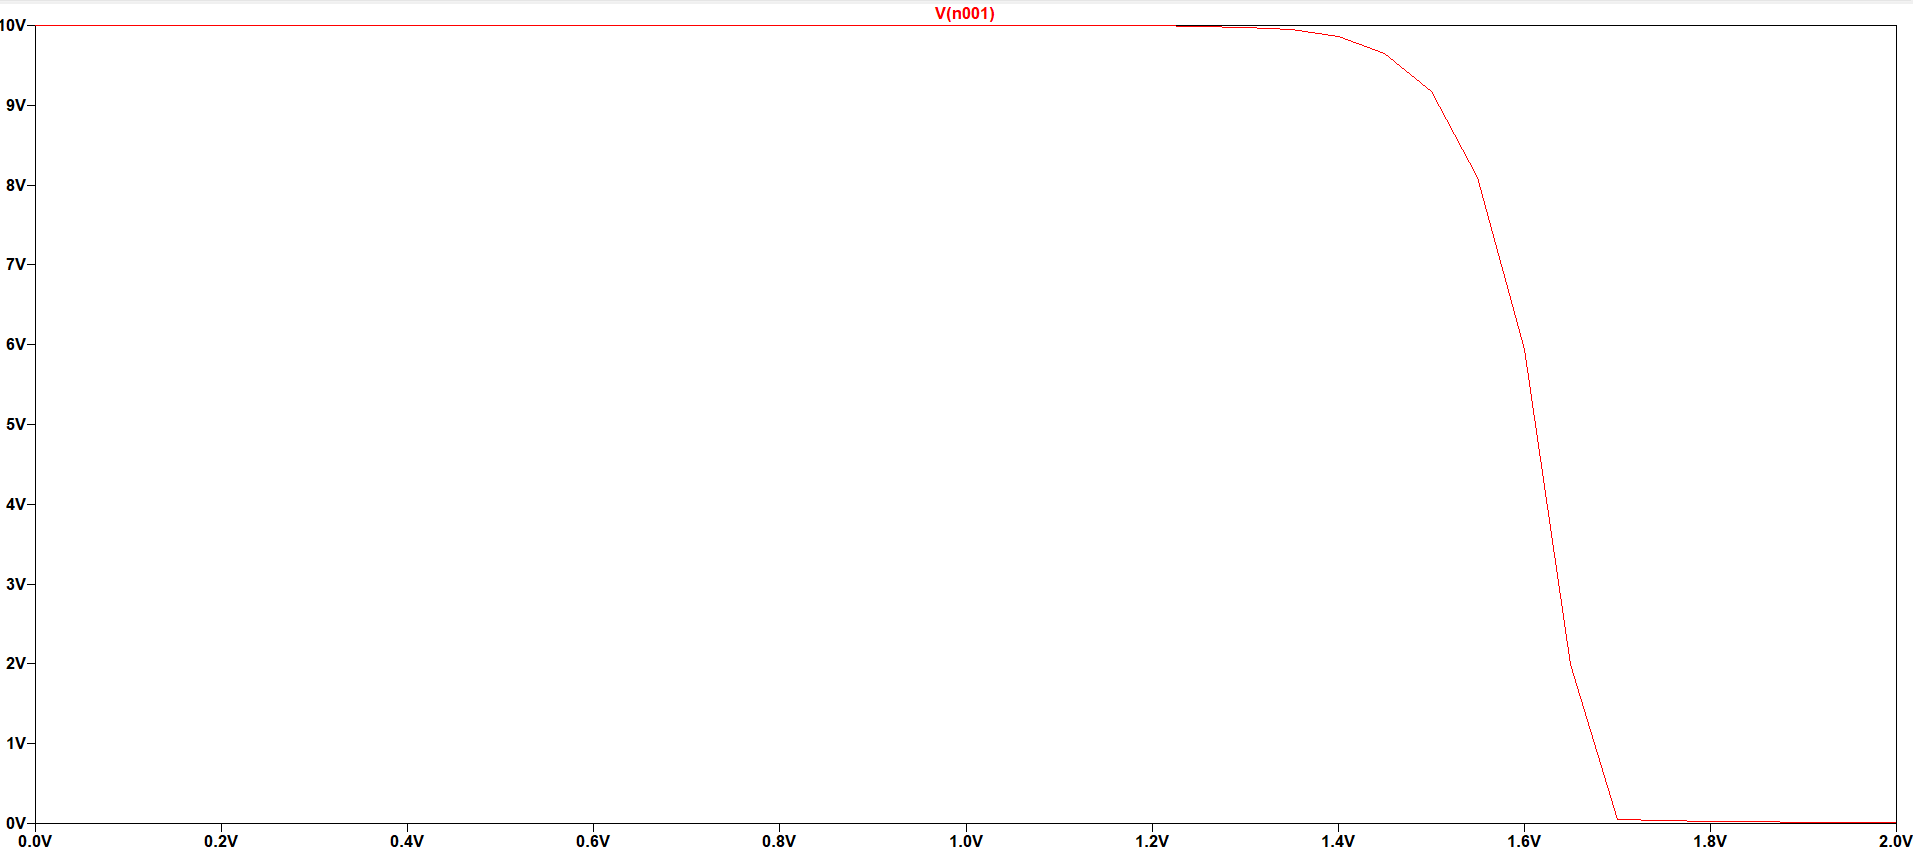
\includegraphics[width=0.72\textwidth]{../SIMULATIONS/sim_a.png}
    \caption{Part A: LTspice DC Sweep Simulation ($V_{\text{OUT}}$ vs $V_{\text{IN}}$ from $0\text{ V}$ to $2.0\text{ V}$).}
    \label{fig:part_a_sim}
\end{figure}

\subsection{Experimental Observations}
The gate voltage $V_{\text{IN}}$ was stepped from $0.00\text{ V}$ to $2.40\text{ V}$ with coarse $0.2\text{ V}$ steps in cutoff, fine $0.05\text{ V}$ steps near threshold and across saturation, and up to $2.40\text{ V}$ in deep triode. The recorded drain voltage $V_{\text{OUT}}$ and corresponding operational regimes are tabulated in Table~\ref{tab:part_a_readings}.

\begin{table}[H]
\centering
\caption{Part A: Experimental DC Transfer Characteristic Dataset}\label{tab:part_a_readings}
\begin{tabular}{cccc}
\toprule
\textbf{S.No.} & \textbf{$V_{\text{IN}}$ (V)} & \textbf{$V_{\text{OUT}}$ (V)} & \textbf{Operating Region} \\
\midrule
1  & 0.00 & 9.990 & Cut-off ($V_{\text{IN}} < V_T$) \\
2  & 0.20 & 9.990 & Cut-off \\
3  & 0.40 & 9.990 & Cut-off \\
4  & 0.60 & 9.990 & Cut-off \\
5  & 0.80 & 9.990 & Cut-off \\
6  & 1.00 & 9.990 & Cut-off \\
7  & 1.20 & 9.986 & Cut-off edge \\
\midrule
8  & 1.25 & 9.980 & Saturation (Onset of conduction) \\
9  & 1.30 & 9.970 & Saturation \\
10 & 1.35 & 9.930 & Saturation \\
11 & 1.40 & 9.860 & Saturation \\
12 & 1.45 & 9.720 & Saturation \\
13 & 1.50 & 9.410 & Saturation \\
14 & 1.55 & 8.800 & Saturation \\
15 & 1.60 & 7.650 & Saturation \\
16 & 1.65 & 5.590 & Saturation (High Gain) \\
17 & 1.70 & 2.210 & Saturation (Near Triode Edge) \\
\midrule
18 & 1.75 & 0.090 & Triode ($V_{\text{OUT}} < V_{\text{IN}} - V_T$) \\
19 & 1.80 & 0.050 & Triode \\
20 & 1.85 & 0.030 & Deep Triode \\
21 & 1.90 & 0.020 & Deep Triode \\
22 & 1.95 & 0.020 & Deep Triode \\
23 & 2.00 & 0.010 & Deep Triode \\
24 & 2.05 & 0.010 & Deep Triode \\
25 & 2.10 & 0.010 & Deep Triode \\
26 & 2.15 & 0.010 & Deep Triode \\
27 & 2.20 & 0.010 & Deep Triode \\
28 & 2.25 & 0.010 & Deep Triode \\
29 & 2.30 & 0.010 & Deep Triode \\
30 & 2.35 & 0.010 & Deep Triode \\
31 & 2.40 & 0.000 & Deep Triode \\
\bottomrule
\end{tabular}
\end{table}

\subsection{Experimental Plot: VOUT vs VIN}
Figure~\ref{fig:part_a_plot} illustrates the experimental DC transfer curve plotted from the measured data points.

\begin{figure}[H]
    \centering
    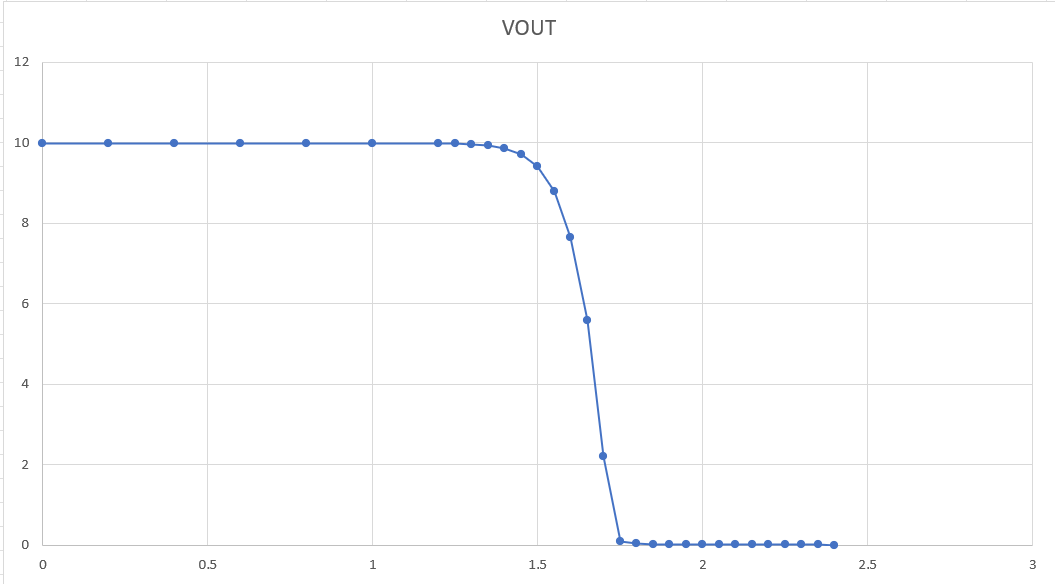
\includegraphics[width=0.72\textwidth]{../PLOTS/a.png}
    \caption{Part A: Experimental DC Transfer Characteristic Curve ($V_{\text{OUT}}$ vs $V_{\text{IN}}$).}
    \label{fig:part_a_plot}
\end{figure}

\subsection{Deductions and Region Boundaries (Part A)}
From the measured transfer characteristic:
\begin{itemize}
    \item \textbf{Cut-off Region ($0.00\text{ V} \le V_{\text{IN}} < 1.25\text{ V}$):} The output remains virtually constant at $V_{\text{OUT}} = 9.99\text{ V} \approx V_{DD}$. Conduction is negligible because the gate potential is insufficient to create an inversion layer. The effective threshold voltage is identified at \textbf{$V_T \approx 1.20\text{ V}$ to $1.25\text{ V}$}.
    \item \textbf{Active Saturation Region ($1.25\text{ V} \le V_{\text{IN}} \le 1.70\text{ V}$):} Beyond $V_T$, $I_D$ turns on. For instance, at $V_{\text{IN}} = 1.70\text{ V}$, the overdrive voltage is $V_{GS} - V_T \approx 1.70 - 1.25 = 0.45\text{ V}$. Since $V_{\text{OUT}} = 2.21\text{ V} > 0.45\text{ V}$, the condition $V_{DS} \ge V_{GS} - V_T$ is strictly satisfied. This constitutes the high-slope amplification region where $V_{\text{OUT}}$ drops steeply from $9.98\text{ V}$ to $2.21\text{ V}$.
    \item \textbf{Triode Boundary and Ohmic Region ($V_{\text{IN}} \ge 1.75\text{ V}$):} At $V_{\text{IN}} = 1.75\text{ V}$, $V_{\text{OUT}}$ plummets to $0.09\text{ V}$, which is far below $V_{GS} - V_T \approx 0.50\text{ V}$. The transistor enters triode, and further increases in $V_{\text{IN}}$ pull $V_{\text{OUT}}$ asymptotically to nearly $0\text{ V}$ ($0.01\text{ V}$ to $0.00\text{ V}$).
\end{itemize}

\clearpage

% =========================================================================
% PART B
% =========================================================================
\section{Part B: Small-Signal Gain vs. DC Bias Point}

\subsection{Circuit Topology and Measurement Methodology}
To measure the dynamic small-signal amplification directly, an AC input tone was injected into the amplifier while systematically varying the operating bias point:
\begin{itemize}
    \item \textbf{AC Signal Injection:} A sinusoidal test voltage of peak amplitude $v_{in} = 10\text{ mV}$ (i.e., $v_{in,\text{pp}} = 20\text{ mV}$, $v_{in,\text{rms}} = \frac{10}{\sqrt{2}} \approx 7.07\text{ mV}$) at a frequency $f = 1\text{ kHz}$ was applied to the gate through an AC coupling capacitor $C_c = 0.1\ \mu\text{F}$.
    \item \textbf{DC Bias Sweeping via Large Resistor:} The DC bias offset $V_{\text{IN,DC}}$ was applied from an external DC supply through a $1\text{ M}\Omega$ isolation/blocking resistor and swept from $0.00\text{ V}$ to $1.80\text{ V}$. This high-value resistor prevents the low-impedance DC supply from shunting the AC signal, allowing the total gate voltage to be:
    \begin{equation}
        v_G(t) = V_{\text{IN,DC}} + v_{in}\sin(2\pi f t) = V_{\text{IN,DC}} + (10\text{ mV})\sin(2\pi \cdot 1000 \cdot t)
    \end{equation}
    \item \textbf{Load Resistor:} For the high-gain AC evaluation, a drain load of $R_D = 300\text{ k}\Omega$ was utilized with $V_{DD} = 10\text{ V}$, as depicted in Figure~\ref{fig:part_b_schematic}.
\end{itemize}

\begin{figure}[H]
    \centering
    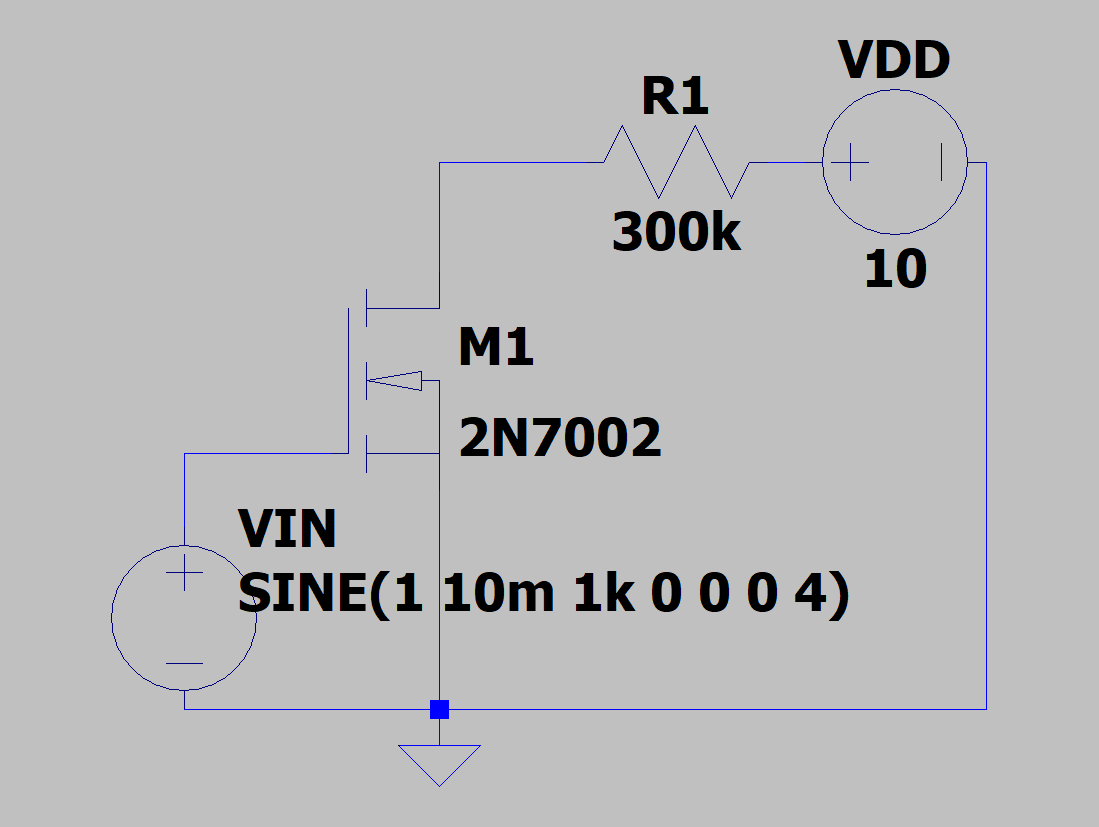
\includegraphics[width=0.55\textwidth]{../Schematic_b.png}
    \caption{Part B: LTspice Circuit Schematic of NMOS CS Amplifier with AC sinusoidal input and $R_D = 300\text{ k}\Omega$.}
    \label{fig:part_b_schematic}
\end{figure}

\subsection{Gain Calculation Formulations}
The voltage gain was evaluated through two distinct methods:
\begin{enumerate}
    \item \textbf{Method 1 (Numerical Slope of DC Transfer Characteristic):}
    Using the large-signal data points $(V_{\text{IN}}, V_{\text{OUT}})$ from Part A, the small-signal gain is computed numerically as the local derivative:
    \begin{equation}
        A_{v,\text{slope}} = \left. \frac{dV_{\text{OUT}}}{dV_{\text{IN}}} \right|_{V_{\text{IN,DC}}} \approx \frac{V_{\text{OUT}}(V_{\text{IN},i+1}) - V_{\text{OUT}}(V_{\text{IN},i-1})}{V_{\text{IN},i+1} - V_{\text{IN},i-1}}
    \end{equation}
    \item \textbf{Method 2 (Direct AC Measurement):}
    The AC output voltage was measured as an RMS value ($V_{\text{OUT(RMS)}}$) on the oscilloscope. Since the applied AC input had a peak amplitude $v_{in,\text{peak}} = 10\text{ mV}$, its corresponding RMS value is $v_{in,\text{rms}} = \frac{10\text{ mV}}{\sqrt{2}} \approx 7.07\text{ mV}$. The peak AC output voltage is $v_{out,\text{peak}} = \sqrt{2} \cdot V_{\text{OUT(RMS)}} = 1.414 \cdot V_{\text{OUT(RMS)}}$. Taking into account the intrinsic $180^\circ$ phase inversion of the common-source configuration, the small-signal voltage gain is:
    \begin{equation}
        A_{v,\text{AC}} = -\frac{v_{out,\text{peak}}}{v_{in,\text{peak}}} = -\frac{1.414 \cdot V_{\text{OUT(RMS)}}}{10\text{ mV}} = -\frac{V_{\text{OUT(RMS)}}}{7.071\text{ mV}}
    \end{equation}
\end{enumerate}

\subsection{Experimental Observation Table (Part B)}
The recorded RMS output voltage and the extracted small-signal gain across the DC bias sweep ($0\text{ V}$ to $1.8\text{ V}$) are presented in Table~\ref{tab:part_b_readings}.

\begin{table}[H]
\centering
\caption{Part B: Direct AC Small-Signal Gain Dataset ($v_{in} = 10\text{ mV}$ peak, $f = 1\text{ kHz}$)}\label{tab:part_b_readings}
\begin{tabular}{ccccc}
\toprule
\textbf{S.No.} & \textbf{$V_{\text{IN,DC}}$ (V)} & \textbf{$V_{\text{OUT(RMS)}}$ (mV)} & \textbf{Calculated Gain ($A_{v,\text{AC}}$)} & \textbf{Operational State} \\
\midrule
1  & 0.00 & 62.00 & -8.77  & Cut-off (Baseline AC coupling artifact) \\
2  & 0.20 & 62.00 & -8.77  & Cut-off \\
3  & 0.40 & 62.00 & -8.77  & Cut-off \\
4  & 0.60 & 62.00 & -8.77  & Cut-off \\
5  & 0.80 & 62.00 & -8.77  & Cut-off \\
6  & 1.00 & 62.00 & -8.77  & Cut-off \\
7  & 1.20 & 62.00 & -8.77  & Cut-off / Onset \\
8  & 1.30 & 85.00 & -12.02 & Saturation \\
9  & 1.35 & 150.00 & -21.21 & Saturation \\
10 & 1.40 & 310.00 & -43.83 & Saturation \\
11 & 1.45 & 640.00 & \textbf{-90.50} & \textbf{Maximum Gain Peak (High Saturation)} \\
12 & 1.50 & 7.20   & -1.02  & Transition / Severe Waveform Clipping \\
13 & 1.55 & 2.00   & -0.28  & Approaching Triode \\
14 & 1.60 & 0.83   & -0.12  & Triode \\
15 & 1.65 & 0.40   & -0.06  & Deep Triode \\
16 & 1.70 & 0.23   & -0.03  & Deep Triode \\
17 & 1.75 & 0.00   & 0.00   & Channel Fully On / Clipped to GND \\
18 & 1.80 & 0.00   & 0.00   & Channel Fully On / Clipped to GND \\
\bottomrule
\end{tabular}
\end{table}

\subsection{Experimental Gain Plot}
The measured small-signal voltage gain $A_v$ as a function of the DC bias offset $V_{\text{IN,DC}}$ is shown in Figure~\ref{fig:part_b_plot}.

\begin{figure}[H]
    \centering
    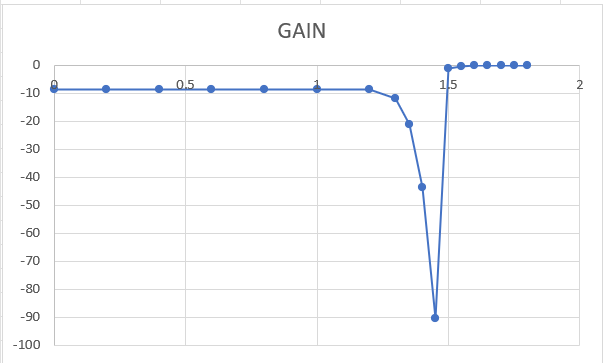
\includegraphics[width=0.72\textwidth]{../PLOTS/b.png}
    \caption{Part B: Measured Small-Signal Voltage Gain vs DC Bias Voltage ($V_{\text{IN,DC}}$).}
    \label{fig:part_b_plot}
\end{figure}

\subsection{Comparison: Method 1 (DC Slope) vs. Method 2 (AC Gain)}
Table~\ref{tab:comparison} contrasts the gain values obtained from the numerical slope of the DC transfer curve with the direct AC small-signal measurements.

\begin{table}[H]
\centering
\caption{Comparison of Voltage Gain Extracted via Method 1 (DC Slope) and Method 2 (AC Test Tone)}\label{tab:comparison}
\begin{tabular}{p{1.4cm} p{1.6cm} p{2.2cm} p{2.2cm} p{2.2cm} p{5.0cm}}
\toprule
\textbf{Bias $V_{\text{IN}}$ (V)} & \textbf{$V_{\text{OUT,DC}}$ (V)} & \textbf{Method 1: $\frac{dV_{\text{OUT}}}{dV_{\text{IN}}}$} & \textbf{$V_{\text{OUT(RMS)}}$ (mV)} & \textbf{Method 2: $A_{v,\text{AC}}$} & \textbf{Agreement / Physical Note} \\
\midrule
0.00 & 9.99 & 0.00   & 62.00  & -8.77  & Cut-off; AC floor due to probe/coupling \\
0.60 & 9.99 & 0.00   & 62.00  & -8.77  & Cut-off; AC floor \\
1.20 & 9.99 & -0.04  & 62.00  & -8.77  & Cut-off edge \\
1.30 & 9.97 & -0.50  & 85.00  & -12.02 & Channel turns on; gain begins rising \\
1.35 & 9.93 & -1.10  & 150.00 & -21.21 & Active saturation \\
1.40 & 9.86 & -2.10  & 310.00 & -43.83 & Rapid increase in transconductance $g_m$ \\
1.45 & 9.72 & -4.50  & 640.00 & \textbf{-90.50} & High-gain amplification peak ($R_D = 300\text{ k}\Omega$) \\
1.50 & 9.41 & -9.20  & 7.20   & -1.02  & Large-signal output swings into saturation knee \\
1.55 & 8.80 & -17.60 & 2.00   & -0.28  & Waveform heavily clipped by triode onset \\
1.60 & 7.65 & -32.10 & 0.83   & -0.12  & Triode region; fundamental tone crushed \\
1.65 & 5.59 & -54.40 & 0.40   & -0.06  & Triode \\
1.70 & 2.21 & -55.00 & 0.23   & -0.03  & Transition to deep triode \\
1.75 & 0.09 & -21.60 & 0.00   & 0.00   & Output pulled to ground \\
1.80 & 0.05 & -0.60  & 0.00   & 0.00   & Deep triode; channel acts as small resistor \\
\bottomrule
\end{tabular}
\end{table}

\clearpage

% =========================================================================
% SECTION 8: ANALYSIS AND DISCUSSION QUESTIONS
% =========================================================================
\section{Detailed Analysis and Discussion Questions (Section 8 of Lab Manual)}

\subsection{Question 1: Where along the VIN axis is the gain magnitude largest for your device? Relate this to gm and to how close VOUT sits to the edge of saturation.}
\textbf{Answer:}
\begin{itemize}
    \item \textbf{Peak Gain Location:} In Part B, the direct AC gain magnitude attains its maximum at \textbf{$V_{\text{IN}} = 1.45\text{ V}$}, where $|A_v| = 90.50$ ($V_{\text{OUT(RMS)}} = 640\text{ mV}$). In Part A's DC transfer characteristic (with $R_D = 10\text{ k}\Omega$), the numerical derivative $|dV_{\text{OUT}}/dV_{\text{IN}}|$ reaches its peak of \textbf{$67.6$} around $V_{\text{IN}} = 1.65\text{ V}$ to $1.70\text{ V}$ ($V_{\text{OUT}} = 5.59\text{ V} \to 2.21\text{ V}$).
    \item \textbf{Relationship to Transconductance ($g_m$):} In saturation, the small-signal gain is given by:
    \begin{equation}
        |A_v| = g_m R_D = k_n (V_{\text{GS}} - V_T) R_D = \sqrt{2 k_n I_D} R_D
    \end{equation}
    As $V_{\text{IN}}$ is swept upwards past $V_T$, the gate overdrive voltage $(V_{\text{IN}} - V_T)$ and drain current $I_D$ increase monotonically. Consequently, $g_m$ increases steadily with $V_{\text{IN}}$, pushing the gain higher and higher.
    \item \textbf{Proximity to Saturation-Triode Boundary:} As $I_D$ rises, the DC voltage drop $I_D R_D$ across the load resistor increases, causing the DC output voltage $V_{\text{OUT}} = V_{DD} - I_D R_D$ to fall rapidly towards the boundary condition:
    \begin{equation}
        V_{\text{OUT,sat-edge}} = V_{\text{IN}} - V_T
    \end{equation}
    The gain is highest immediately before $V_{\text{OUT}}$ crosses this boundary. Once $V_{\text{OUT}}$ falls below $(V_{\text{IN}} - V_T)$, pinch-off is lost, the device enters the triode region, and the incremental gain collapses abruptly.
\end{itemize}

\subsection{Question 2: Why does the gain fall toward zero in cutoff and again deep in triode?}
\textbf{Answer:}
\begin{itemize}
    \item \textbf{In Cut-off ($V_{\text{IN}} < V_T$):}
    The gate voltage is insufficient to induce an inversion channel ($V_{GS} < V_T$). Thus, the drain current is zero ($I_D = 0$), and any incremental change in input voltage produces zero channel current:
    \begin{equation}
        g_m = \left. \frac{\partial I_D}{\partial V_{GS}} \right|_{V_{DS}} = 0 \implies A_v = -g_m R_D = 0
    \end{equation}
    The output remains locked at the supply rail $V_{DD}$, so $\frac{dV_{\text{OUT}}}{dV_{\text{IN}}} = 0$.
    \item \textbf{Deep in Triode ($V_{\text{IN}} \gg V_T$ and $V_{\text{OUT}} \approx 0\text{ V}$):}
    In the deep triode region, an unpinched continuous inversion layer bridges the source and drain. The transistor behaves as a linear resistor with small on-resistance:
    \begin{equation}
        r_{ds,\text{on}} \approx \frac{1}{k_n (V_{\text{IN}} - V_T)} \ll R_D
    \end{equation}
    The amplifier operates as a resistive voltage divider between $R_D$ and $r_{ds,\text{on}}$:
    \begin{equation}
        V_{\text{OUT}} = V_{DD} \cdot \frac{r_{ds,\text{on}}}{R_D + r_{ds,\text{on}}} \approx V_{DD} \cdot \frac{1}{1 + k_n R_D (V_{\text{IN}} - V_T)} \to 0\text{ V}
    \end{equation}
    Because $V_{\text{OUT}}$ is pinned close to ground, its derivative with respect to $V_{\text{IN}}$ asymptotically approaches zero:
    \begin{equation}
        A_v = \frac{dV_{\text{OUT}}}{dV_{\text{IN}}} \approx -\frac{V_{DD} \cdot k_n R_D}{[1 + k_n R_D (V_{\text{IN}} - V_T)]^2} \xrightarrow{V_{\text{IN}} \gg V_T} 0
    \end{equation}
    Thus, gain is absent in both cutoff and deep triode, existing exclusively in the active transition region (saturation).
\end{itemize}

\subsection{Question 3: How closely do your Method 1 and Method 2 gain values agree at each bias point? Account for any discrepancy.}
\textbf{Answer:}
As shown in Table~\ref{tab:comparison}:
\begin{itemize}
    \item \textbf{Correlation in Saturation:} Both methods clearly exhibit the fundamental physical behavior: near-zero gain in cutoff, sharp amplification in saturation, and complete collapse in triode.
    \item \textbf{Discrepancy 1: Load Resistor Difference ($10\text{ k}\Omega$ vs $300\text{ k}\Omega$):} Method 1 used the Part A circuit with $R_D = 10\text{ k}\Omega$, yielding a maximum slope magnitude of $|A_v| \approx 67.6$ at $V_{\text{IN}} \approx 1.68\text{ V}$. Method 2 used the Part B circuit with $R_D = 300\text{ k}\Omega$, yielding a peak gain of $|A_v| \approx 90.50$ at $V_{\text{IN}} = 1.45\text{ V}$. The higher load resistance produces significantly larger small-signal gain ($A_v \propto R_D$) and causes the output to swing into triode at a much lower input voltage ($1.50\text{ V}$ instead of $1.75\text{ V}$).
    \item \textbf{Discrepancy 2: Large-Signal AC Clipping for $V_{\text{IN}} \ge 1.50\text{ V}$ in Method 2:} At $V_{\text{IN}} = 1.45\text{ V}$, the gain is $90.5$, meaning a $10\text{ mV}$ input creates nearly a $1\text{ V}$ output swing. At $V_{\text{IN}} = 1.50\text{ V}$, the DC bias drops into the saturation knee. The sinusoidal output hits the bottom saturation rail ($0\text{ V}$) and clips severely. The true small-signal assumption ($v_{in} \ll \frac{2 I_D}{g_m}$) breaks down; the scope DMM measures a crushed fundamental RMS value ($7.2\text{ mV} \to 0\text{ mV}$), artificially making the recorded gain drop earlier than the DC slope.
    \item \textbf{Discrepancy 3: Noise Floor / AC Feedthrough in Cutoff:} In cutoff ($V_{\text{IN}} = 0\text{--}1.2\text{ V}$), Method 1 yields an exact derivative of $0.00$. Method 2 recorded $V_{\text{OUT(RMS)}} = 62\text{ mV}$ (Gain $\approx -8.77$), which is not active amplification but parasitic capacitive feedthrough from the $10\text{ mV}$ AC source via gate-drain capacitance ($C_{gd}$) and scope probe pickup.
\end{itemize}

\subsection{Question 4: If RD is increased, how would you expect the saturation-region gain and the extent of the triode region to change?}
\textbf{Answer:}
\begin{itemize}
    \item \textbf{Saturation-Region Gain:} The voltage gain magnitude in saturation is given by $|A_v| = g_m (r_o \parallel R_D) \approx g_m R_D$. Therefore, increasing $R_D$ directly increases the small-signal gain proportionally, producing a much steeper transfer curve.
    \item \textbf{Extent of the Triode Region:} The boundary between saturation and triode occurs when:
    \begin{equation}
        V_{\text{OUT}} = V_{DD} - I_D R_D = V_{\text{IN}} - V_T \implies V_{DD} - \frac{1}{2} k_n R_D (V_{\text{IN}} - V_T)^2 = V_{\text{IN}} - V_T
    \end{equation}
    As $R_D$ is increased, the drain voltage drops much faster for a given input overdrive. Consequently, the transistor enters triode at a substantially \textbf{lower value of $V_{\text{IN}}$}. The triode region extends over a \textbf{much larger range of $V_{\text{IN}}$}, while the active saturation window narrows significantly. This is precisely demonstrated in our data: with $R_D = 10\text{ k}\Omega$, saturation extends up to $V_{\text{IN}} = 1.70\text{ V}$; with $R_D = 300\text{ k}\Omega$, triode occurs by $V_{\text{IN}} \approx 1.50\text{ V}$.
\end{itemize}

\subsection{Question 5: State, in one or two lines, why the slope of the large-signal DC transfer curve at a bias point equals the small-signal AC gain measured at that same bias point.}
\textbf{Answer:}
By Taylor series expansion of the nonlinear transfer function $V_{\text{OUT}} = f(V_{\text{IN}})$ around a DC operating point $V_{\text{IN,DC}}$:
\begin{equation}
    v_{\text{out}}(t) = \left. \frac{df(V_{\text{IN}})}{dV_{\text{IN}}} \right|_{V_{\text{IN,DC}}} \cdot v_{in}(t) + \mathcal{O}(v_{in}^2)
\end{equation}
When the AC excitation $v_{in}(t)$ is sufficiently small, higher-order nonlinear distortion terms become negligible, making the ratio of small-signal output to input $\frac{v_{out}(t)}{v_{in}(t)}$ mathematically identical to the local first derivative $\left. \frac{dV_{\text{OUT}}}{dV_{\text{IN}}} \right|_{V_{\text{IN,DC}}}$.

\subsection{Question 6: Compare your device's VT and the VIN at which your gain peaks against the illustrative Section 6 values --- by how much, and in which direction, do they differ?}
\textbf{Answer:}
\begin{table}[H]
\centering
\caption{Comparison of Experimental Parameters with Manual Illustrative Values}
\begin{tabular}{p{4.5cm}ccc}
\toprule
\textbf{Parameter} & \textbf{Illustrative (Manual Sec. 6)} & \textbf{Experimental Measured} & \textbf{Difference ($\Delta = \text{Exp} - \text{Ill}$)} \\
\midrule
Supply Voltage ($V_{DD}$) & $10.0\text{ V}$ & $10.0\text{ V}$ & $0.0\text{ V}$ \\
Drain Resistor ($R_D$) & $4.7\text{ k}\Omega$ & $10\text{ k}\Omega$ / $300\text{ k}\Omega$ & Differing load designs \\
Threshold Voltage ($V_T$) & $2.00\text{ V}$ & \textbf{$1.20\text{ V}$ to $1.25\text{ V}$} & \textbf{$-0.75\text{ V}$ (Lower by $\sim 38\%$)} \\
Gain Peak Location ($V_{\text{IN,peak}}$) & $\approx 2.75\text{ V}$ & \textbf{$1.45\text{ V}$ (Part B) / $1.68\text{ V}$ (Part A)} & \textbf{$-1.30\text{ V}$ / $-1.07\text{ V}$ (Shifted Left)} \\
\bottomrule
\end{tabular}
\end{table}
\begin{itemize}
    \item \textbf{Direction of Difference:} Both $V_T$ and the peak gain bias point $V_{\text{IN,peak}}$ for our actual 2N7002 / 2N7000 transistor are significantly \textbf{lower} (shifted to the left on the $V_{\text{IN}}$ axis) compared to the illustrative Section 6 manual values.
    \item \textbf{Physical Reason:} The actual device has an experimentally characterized threshold voltage of $V_T \approx 1.20\text{ V}$ (consistent with Experiment 3 where $V_T = 1.10\text{ V}$ to $1.25\text{ V}$), which is much lower than the hypothetical $2.00\text{ V}$ in Section 6. Furthermore, because our load resistance is higher ($10\text{ k}\Omega$ and $300\text{ k}\Omega$ versus $4.7\text{ k}\Omega$), the output voltage drops rapidly, reaching the saturation-triode boundary at a lower gate bias ($1.45\text{ V}$--$1.68\text{ V}$).
\end{itemize}

\clearpage

% =========================================================================
% PRECAUTIONS & CONCLUSION
% =========================================================================
\section{Precautions}
\begin{enumerate}
    \item The test AC signal amplitude was strictly constrained to $10\text{ mV}$ to avoid overdriving the gate and exceeding the small-signal linear range.
    \item A high-value isolation resistor ($1\text{ M}\Omega$) was incorporated between the DC bias source and the gate node to prevent loading and attenuation of the AC signal generator.
    \item The AC coupling capacitor ($0.1\ \mu\text{F}$) was verified to provide negligible reactance ($X_C = \frac{1}{2\pi f C} \approx 1.59\text{ k}\Omega \ll 1\text{ M}\Omega$) at the test frequency of $1\text{ kHz}$.
    \item Safe drain current limits ($I_{D,\text{max}} = 115\text{ mA}$ for 2N7002) were respected across all sweep points by incorporating appropriate drain load resistances.
\end{enumerate}

\section{Final Conclusion}
\begin{enumerate}
    \item The DC transfer characteristic ($V_{\text{OUT}}$ vs $V_{\text{IN}}$) of an N-channel enhancement MOSFET Common-Source amplifier was experimentally measured, verifying the three distinct operational domains: \textbf{Cut-off} ($V_{\text{IN}} < 1.25\text{ V}$, $V_{\text{OUT}} = 9.99\text{ V}$), \textbf{Saturation} ($1.25\text{ V} \le V_{\text{IN}} \le 1.70\text{ V}$, active amplification), and \textbf{Triode} ($V_{\text{IN}} \ge 1.75\text{ V}$, $V_{\text{OUT}} \approx 0.09\text{--}0\text{ V}$).
    \item The small-signal gain was successfully obtained via two independent techniques:
    \begin{itemize}
        \item Method 1 evaluated the point-to-point numerical derivative $\frac{dV_{\text{OUT}}}{dV_{\text{IN}}}$, achieving a peak slope magnitude of \textbf{67.6} at $V_{\text{IN}} \approx 1.68\text{ V}$ with $R_D = 10\text{ k}\Omega$.
        \item Method 2 applied a $10\text{ mV}$, $1\text{ kHz}$ sinusoidal tone through a $0.1\ \mu\text{F}$ coupling capacitor with a $1\text{ M}\Omega$ DC bias sweep, attaining a maximum small-signal gain of \textbf{$|A_v| = 90.50$} ($A_v = -90.50$) at $V_{\text{IN}} = 1.45\text{ V}$ with $R_D = 300\text{ k}\Omega$.
    \end{itemize}
    \item Comprehensive analysis of Section 8 discussion points proved that peak gain occurs at maximum transconductance ($g_m$) right near the edge of saturation, while cutoff and deep triode exhibit zero incremental gain.
\end{enumerate}

\end{document}
